\chapter{Introduction}
\label{introduction}
Current Internet architecture based mostly on TCP/IP stack allows establishing communication channels between two IP addresses. While this model worked for past years, now it struggles to fit current demands. Today the Internet is dominated by transporting content such as audio, video, images, and text from content creators to content consumers. Information-centric networks introduce a paradigm shift from a host-oriented to a content-oriented paradigm. By placing content in the center of interest, it allows for achieving several benefits. All network participants become more aware of transferring content. This kind of awareness allows implementing various improvements over host-based paradigms such as content caching, mobility, integrity, and security assurance. All of those features are guaranteed natively by an ICN transport layer.

Many projects implement the ICN approach: Data-Oriented Network Architecture (DONA), Named Data Networking (NDN), Publish-Subscribe Network Technology (PURSUIT), Scalable and Adaptable Network Solutions (SAIL), Inter-planetary File System (IPFS).

They all differ in details, but the core concepts are the same, they try to achieve a pull-driven communication model suited for disconnections, disruptions, mobility, and transferring large data to many devices. They introduce in-network storage on each node for data caching. Also, decouple senders from receivers by resolving content by its name––not a host's location. 
In ICN, a data piece is requested by its name (Named Data Object - NDO) and is served by the closest possible node that is storing it, allowing efficient caching on the transport layer––relieving an application layer from implementing a cache strategy individually.

When we write NDO, we understand any arbitrary data piece that can be transferred over the network: a web page, music, images, video, documents, and data streams. Most importantly, NDOs, compared to traditional URLs, are location independent. They do not specify the location where the content should be served from, nor how it should be transferred to the receiver. NDO granularity may differ from packets to data chunks to whole data objects, depending on the approach and data size.

Data naming is the most significant concept in ICN. Data names must be unique––similarly to hostnames in current Internet architecture; two different DNS nodes must resolve one domain name to the same location––two different ICN nodes must resolve one name to the same content. 
There are two approaches to a naming system: 1) hierarchical - similar to URL, and 2) flat - global namespace, often just a hash of the file.
Additionally, each NDO should be authenticated by the publisher who created it. Digital signatures on data objects guarantee both integrity and authentication. If a data piece is trusted, not the host, then it can be served from any untrusted source––and we still can trust it.

The most significant benefit of ICN networks is content caching. It turns out that this benefit becomes a double-edged sword when we take into account security concerns. If everything that makes a content authentic is a valid signature, an intruder who gets access to the publisher's private key can create poisoned content with valid signatures. Such content can be easily disseminated to ICN nodes, but hardly removed due to the lack of removal operation in ICN architecture. 

This thesis aims to provide a mechanism to protect subscribers from trusting poisoned content, even in situations when an intruder has access to a stolen private key (making it indistinguishable from the actual publisher).

This thesis contributes to the field of ICN networking by 
\begin{enumerate}
    \item Formulating the general approach to protect a subscriber from a content poisoning attack.
    \item Building simulators that allow analyzing a graph infection implementation proposed by \cite{konorski2019mitigating}. 
    \item Observing a Defensive Alliance phenomenon that causes problems in the GI algorithm.
    \item Proposing a new implementation based on Blockchain technology.
    \item Evaluating and comparing those two approaches in the context of scalability, complexity, fault-tolerance, and resiliency. 
\end{enumerate}

The remainder of this thesis is organized as follows.
In Sec. \ref{ndn}, we present an example project implementing ICN architecture; we decided on Named Data Networking (NDN) since it is the most popular one.
In Sec. \ref{content-poisoning}, we describe a problem of Content Poisoning Attacks and in Sec. \ref{proof-of-time} and \ref{network-structure} an approach to solve it. In Sec. \ref{epidemiology} we study epidemiology models to get intuition to graph infection algorithm proposed in \cite{konorski2019mitigating} and described in Sec. \ref{graph-infection}. Then in Sec. \ref{simulator}, we describe simulators used to analyze the algorithm and in Sec. \ref{observations} observations that show weaknesses of such an algorithm. In Sec. \ref{consensus}, we generalize our initial problem to a consensus problem, which we then solve by using Blockchain technology and Federated Byzantine Agreement consensus protocol (described in Chapter \ref{blockchain}). Finally, a comparison of both protocols is presented in Sec. \ref{comparison}.

\section{Named Data Networking}
\label{ndn}
To get a better understanding of how ICN networks work, we describe one of the most mature projects. The design was initially proposed under the name Content-Centric Network by Van Jacobson in 2006 \cite{4ANewWay38:online}. Currently, the project is under development with the name Named Data Networking (NDN) \cite{NamedDat22:online}. 

NDN replace TCP/IP protocol stack by placing chunks of named content in place of IP addresses (see Fig \ref{fig:ndn-design}a). The only layer that cannot be changed is the layer 3––the thin "waist" of the stack. All protocols in the rest of the layers can be adjusted to the needs.
\begin{figure}[h!]
  \subfloat[]{
	\begin{minipage}[c][\width]{
	   0.49\textwidth}
	   \centering
	   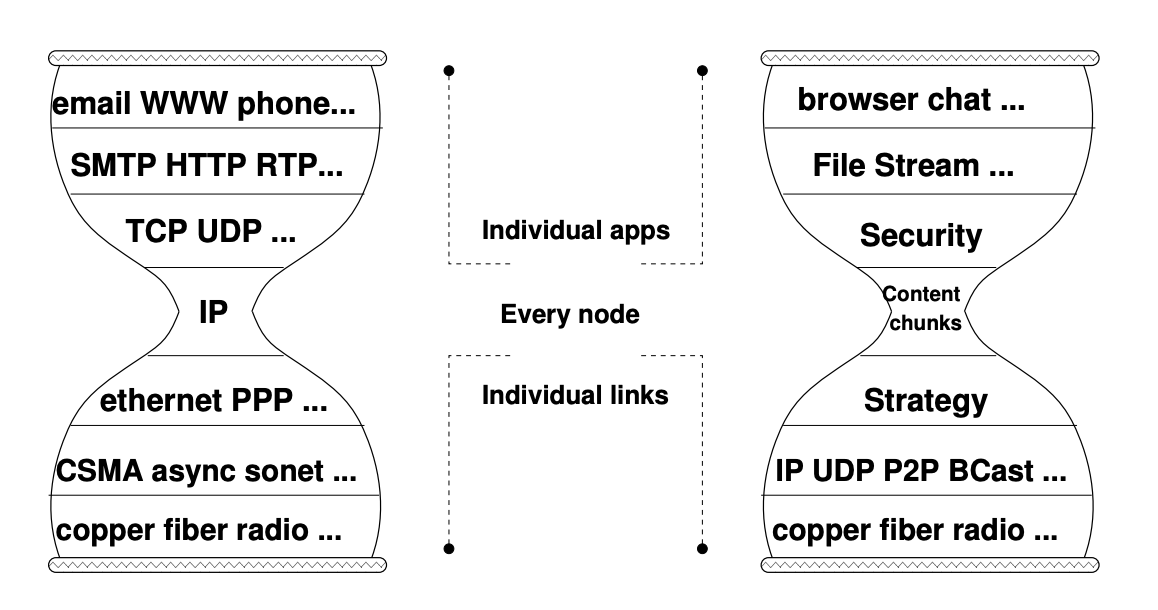
\includegraphics[width=1\textwidth]{img/ndn-stack.png}
	\end{minipage}}
 \hfill 	
  \subfloat[]{
	\begin{minipage}[c][\width]{
	   0.49\textwidth}
	   \centering
	   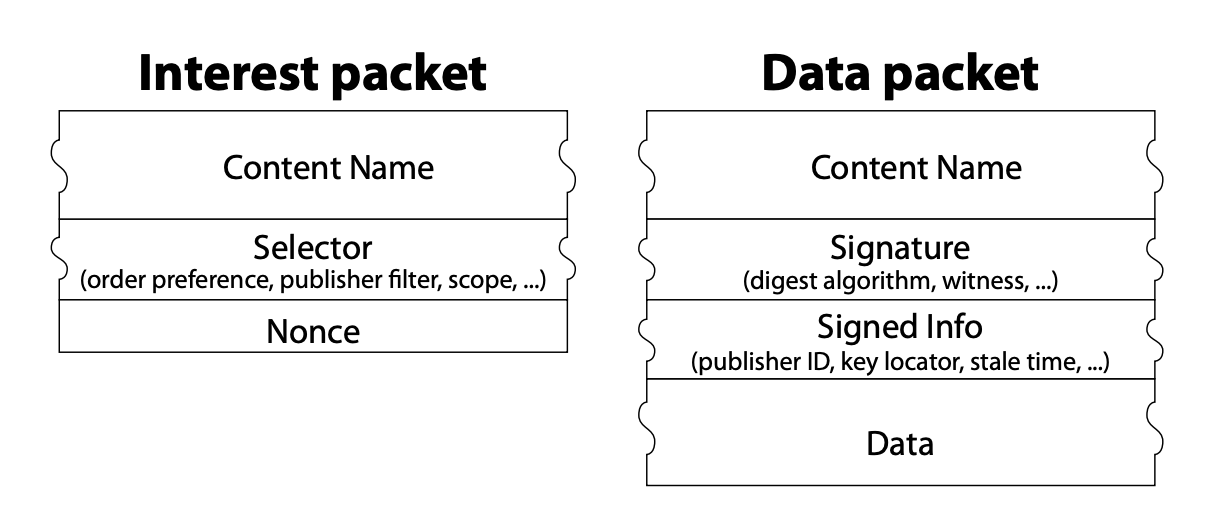
\includegraphics[width=1\textwidth]{img/ndn-packets.png}
	\end{minipage}}
\caption{Named Data Networking design. Source \cite{jacobson2009networking}}
\label{fig:ndn-design}
\end{figure}
NDN defines two types of packets: Interest, and Data (see Fig. \ref{fig:ndn-design}b). An Interest packet, as the name suggests, indicate a interest of some data chunk, where a data chunk is identified by its Content Name. A consumer broadcasts an Interest packet to all its connection faces. If any node that receives such a message has the corresponding data locally, it can respond with a Data Packet, otherwise the Interest is forwarded to next router. In Fig. \ref{fig:ndn-operations} we can see the forward engine model in NDN node. When a request arrives at one of available faces it gets dispatched based on the lookup result. 

\begin{itemize}
    \item FIB (Forwarding Information Base) is responsible for forwarding the interests to potential nodes where the data can be found (similar to FIB used in IP, except it allows for multiple outgoing faces rather than a single one). 

    \item Content Store(CS) is responsible for buffering content requested by the Interest packet. Since the data can be served to multiple consumers–––not just a single connection, as it is done in IP––it is not recycled after the first Interest request is satisfied. This mechanism is called in-network storage because the network itself is storing the data. It is possible due to idempotency, self-identification, and self-authentication of packets, so each packet is equally useful for many consumers (e.g., two hosts interesting in Netflix video can receive content from a single node without requesting the Netflix servers). Data is stored as long as possible, and different storage policies can be used, e.g., LRU replacement.

    \item PIT (Pending Interest Table) stores information about the interests forwarded to potential data sources. When one of them replies with a Data packet, the PIT is checked if some consumer is waiting for the data, and if so, the Data packet is forwarded to corresponding face.
\end{itemize}
\begin{figure}[h]
    \centering
    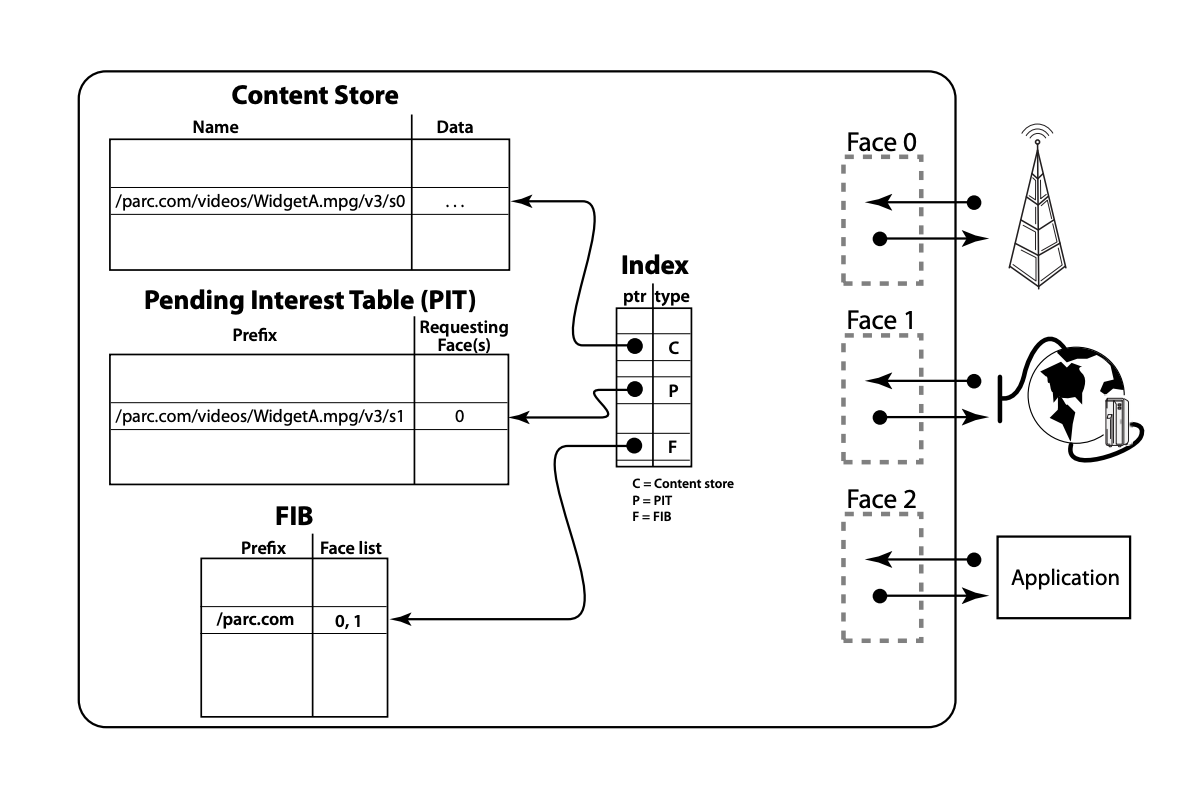
\includegraphics[width=\linewidth]{img/ndn-operations.png}
    \caption{NDN node operations. Source \cite{jacobson2009networking}}
    \label{fig:ndn-operations}
\end{figure}
To better understand the model, a concrete packet flow is presented in Fig.\ref{fig:ndn-flow}. 
\begin{enumerate}
    \item A requester application wants to receive some data. It sends a request to its local NDN engine. The node first checks the local CS, and since the content is absent, it requests the Interest packet to the closes router.
    \item The router first checks its Content Store, and if the data is absent, it checks if there is already a pending interest in the PIT for such data. If not, the request is forwarded to the next router, according to FIB.  
    \item The next router does the same as the previous router. It checks its CS, PIT, and then forward the Interest packet through FIB.
    \item Finally, the Interest reaches the data source router, where the content is present in the CS, so it is immediately returned.
    \item The router receives the Data packet and stores it in its CS, check which nodes are waiting for the data in PIT and forwards the Data packet accordingly.
    \item This router (initially requested by the requestor) does the same as the previous router, storing the data in CS and responding with the Data packet.
    \item After some time, the different requester sends the Interest packet to its closest router.
    \item Router looks up the Content Name and finds out that the content is already stored in CS. Therefore it immediately returns the Data packet to save the network bandwidth and reducing the latency.
\end{enumerate}

\begin{figure}[h]
    \centering
    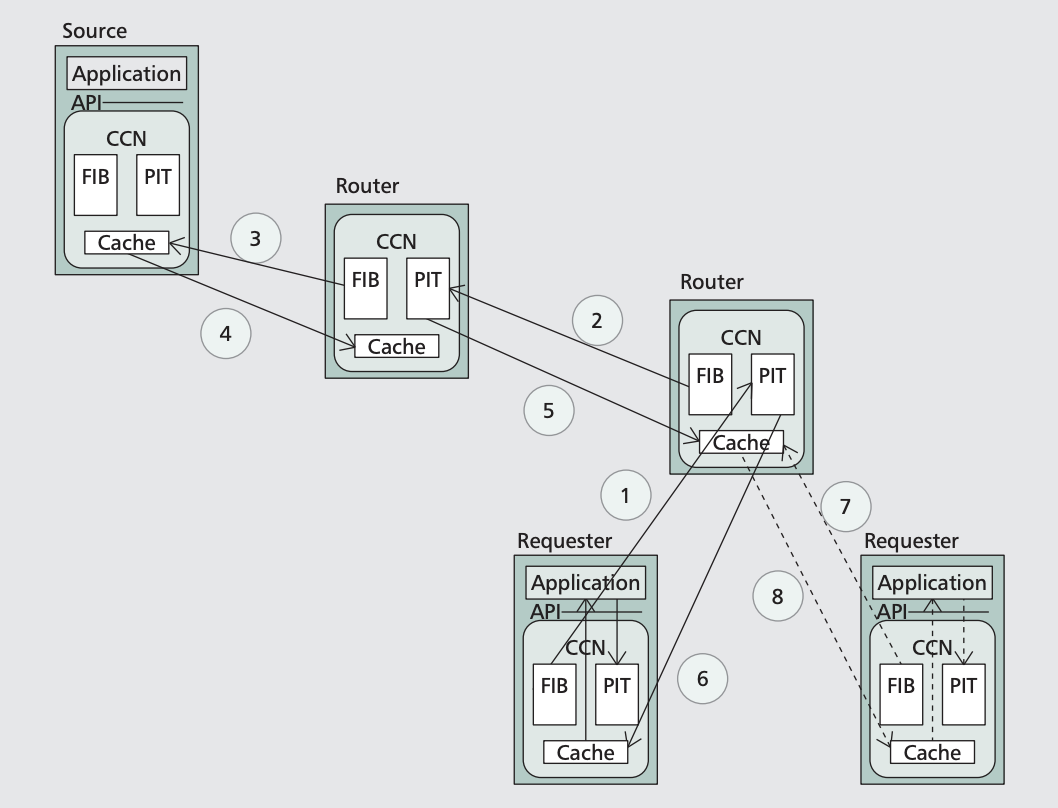
\includegraphics[width=\linewidth]{img/ndn-flow.png}
    \caption{NDN packets flow. Source \cite{ahlgren2012survey}}
    \label{fig:ndn-flow}
\end{figure}